\documentclass[11pt,]{article}
\usepackage[]{mathpazo}
\usepackage{amssymb,amsmath}
\usepackage{ifxetex,ifluatex}
\usepackage{fixltx2e} % provides \textsubscript
\ifnum 0\ifxetex 1\fi\ifluatex 1\fi=0 % if pdftex
  \usepackage[T1]{fontenc}
  \usepackage[utf8]{inputenc}
\else % if luatex or xelatex
  \ifxetex
    \usepackage{mathspec}
  \else
    \usepackage{fontspec}
  \fi
  \defaultfontfeatures{Ligatures=TeX,Scale=MatchLowercase}
\fi
% use upquote if available, for straight quotes in verbatim environments
\IfFileExists{upquote.sty}{\usepackage{upquote}}{}
% use microtype if available
\IfFileExists{microtype.sty}{%
\usepackage{microtype}
\UseMicrotypeSet[protrusion]{basicmath} % disable protrusion for tt fonts
}{}
\usepackage{hyperref}
\PassOptionsToPackage{usenames,dvipsnames}{color} % color is loaded by hyperref
\hypersetup{unicode=true,
            colorlinks=true,
            linkcolor=black,
            citecolor=black,
            urlcolor=black,
            breaklinks=true}
\urlstyle{same}  % don't use monospace font for urls
\usepackage{natbib}
\bibliographystyle{EcolLett}
\usepackage{graphicx,grffile}
\makeatletter
\def\maxwidth{\ifdim\Gin@nat@width>\linewidth\linewidth\else\Gin@nat@width\fi}
\def\maxheight{\ifdim\Gin@nat@height>\textheight\textheight\else\Gin@nat@height\fi}
\makeatother
% Scale images if necessary, so that they will not overflow the page
% margins by default, and it is still possible to overwrite the defaults
% using explicit options in \includegraphics[width, height, ...]{}
\setkeys{Gin}{width=\maxwidth,height=\maxheight,keepaspectratio}
\IfFileExists{parskip.sty}{%
\usepackage{parskip}
}{% else
\setlength{\parindent}{0pt}
\setlength{\parskip}{6pt plus 2pt minus 1pt}
}
\setlength{\emergencystretch}{3em}  % prevent overfull lines
\providecommand{\tightlist}{%
  \setlength{\itemsep}{0pt}\setlength{\parskip}{0pt}}
\setcounter{secnumdepth}{0}
% Redefines (sub)paragraphs to behave more like sections
\ifx\paragraph\undefined\else
\let\oldparagraph\paragraph
\renewcommand{\paragraph}[1]{\oldparagraph{#1}\mbox{}}
\fi
\ifx\subparagraph\undefined\else
\let\oldsubparagraph\subparagraph
\renewcommand{\subparagraph}[1]{\oldsubparagraph{#1}\mbox{}}
\fi

%%% Use protect on footnotes to avoid problems with footnotes in titles
\let\rmarkdownfootnote\footnote%
\def\footnote{\protect\rmarkdownfootnote}

%%% Change title format to be more compact
\usepackage{titling}

% Create subtitle command for use in maketitle
\providecommand{\subtitle}[1]{
  \posttitle{
    \begin{center}\large#1\end{center}
    }
}

\setlength{\droptitle}{-2em}

  \title{}
    \pretitle{\vspace{\droptitle}}
  \posttitle{}
    \author{}
    \preauthor{}\postauthor{}
    \date{}
    \predate{}\postdate{}
  
\usepackage{fullpage}
\linespread{1.5}
\usepackage{lineno}
\usepackage{caption,setspace}
\captionsetup[figure]{font=small}

\begin{document}

\vspace*{0.1cm}

\begin{center} \LARGE Ecological character displacement destabilizes food webs \end{center}

\bigskip

\begin{center} \large Matthew A. Barbour$^{1,2,\ast}$ \normalsize \end{center}

\bigskip

\noindent 1. University of Zurich, Department of Evolutionary Biology
and Environmental Studies, Winterthurerstrasse 190, 8057 Zurich,
Switzerland;

\noindent 2. University of British Columbia, Department of Zoology, 2212
Main Mall, Vancouver, BC V6T 1Z4, Canada;

\(^\ast\) Corresponding author; e-mail:
\href{mailto:matthew.barbour@ieu.uzh.ch}{\nolinkurl{matthew.barbour@ieu.uzh.ch}},
phone: +41 44 635 61 63

\bigskip

\emph{Statement of authorship}: MAB conceived the study, derived
analytical solutions, performed simulations, and wrote the paper.

\bigskip

\emph{Data accessibility}: No new data were used. All code used to
reproduce this manuscript and simulations within are publically
available on GitHub (\url{https://github.com/mabarbour/ECD_model}).

\bigskip

\emph{Running title}: Character displacement destabilizes food webs

\bigskip

\emph{Keywords}: competition; eco-evolutionary dynamics;
consumer-resource interactions; adaptation; community stability

\linenumbers{} \modulolinenumbers[3]

\newpage

\section{Abstract}\label{abstract}

Ecological character displacement is an adaptive process that generally
increases phenotypic diversity. Despite the fact that this
diversification is due to an eco-evolutionary feedback between consumers
competing for shared resources, its consequences for food-web dynamics
have received little attention. Here, I study a model of two consumers
competing for two shared resources to examine how character displacement
in consumer attack rates affects resource abundances and the resilience
of food webs to perturbations. I found that character displacement
always strengthened consumer-resource interactions whenever consumers
competed for resources that occurred in different habitats. This
increase in interaction strength resulted in lower resource abundances
and less resilient food webs. This occurred under different evolutionary
tradeoffs and in both simple and more realistic foraging scenarios.
Taken together, my results show that the adaptive process of character
displacement may come with the ecological cost of decreasing food-web
resilience.

\newpage

\section{Introduction}\label{introduction}

Ecological character displacement is an important adaptive process in
generating biodiversity \citep{Schluter2000, Pfennig2010}. This process
is due to ``phenotypic evolution in a species generated or maintained by
{[}exploitative{]} resource competition with one or more coexisting
species'' \citep{Schluter2000}. A large body of theoretical
\citep[e.g.][]{Lawlor1976, Abrams1986, Doebeli1996, Taper1985, McPeek2019}
and empirical \citep[reviewed
in:][]{Schluter2000, Dayan2005, Stuart2013} work has examined which
scenarios lead to phenotypic divergence or convergence of competing
consumers. The general conclusion has been that, if resources are
nutritionally substitutable \citep{Abrams1987, Fox2008} and there is no
other strong source of density dependence acting on consumers
\citep{Abrams1986}, then resource competition drives the adaptive
divergence of competitors \citep{Lawlor1976, Taper1985}. This adaptive
process is not simply a response to static differences in resource
distributions, but creates an eco-evolutionary feedback that drives
further differentiation. This crucial insight was made by theoretical
models that explicitly included resource dynamics as a mediator of
competition in driving evolutionary change
\citep{Lawlor1976, Abrams1986, Taper1985}.

Although models that included resources led to insights about the
evolution of character displacement, the ecological feedback onto
consumer-resource dynamics has received surprisingly little attention.
This is likely because the ecological feedback has been primarily
studied through the lens of coexistence theory
\citep{Lawlor1976, Germain2018, Bassar2017, McPeek2019}. For example,
early theoretical work showed that character displacement promotes
coexistence by favoring specialized consumers that experience reduced
interspecific competition \citep{Lawlor1976}. Yet, this reduction in
interspecific competition may, at the same time, increase interspecific
interactions between specialized consumers and their resources. Both
food-web theory and empirical studies have shown that increasing the
strength of consumer-resource interactions often suppresses the
abundance of resources, which if sufficient enough, can generate
oscillations and less stable consumer-resource dynamics
\citep{Rosenzweig1971, Luckinbill1973, Murdoch2002, Murdoch2003, McCann2011}.
Thus, a food-web perspective, which accounts for both the direct and
indirect effects of consumer-resource interactions, may yield new
insight to the ecological consequences of character displacement.

Here, I address this knowledge gap by studying a mathematical model that
examines how ecological character displacement affects consumer-resource
dynamics in a food-web context. Specifically, I sought to answer the
question: how does character displacement in consumer attack rates
affect resource abundances and food-web stability? To test the
generality of these effects, I explored different ecological foraging
scenarios and evolutionary tradeoffs in consumer attack rates. I found
that the adaptive process of character displacement often comes with an
ecological cost; resulting in food webs with lower resource availability
and that are less resilient to perturbations.

\section{Material and methods}\label{material-and-methods}

\subsection{Underlying consumer-resource
dynamics}\label{underlying-consumer-resource-dynamics}

To examine how ecological character displacement affects resource
abundances and food-web stability, I analyzed a continuous-time model of
two consumers (\(C_{j=1,2}\)) competing for two shared resources
(\(R_{i=1,2}\)):

\begin{equation} \label{eq:1}
  \begin{split}
     & \frac{dR_1}{dt}=r_1R_1(1-\frac{R_1}{K_1})-F_{11}(R_1)C_1-F_{12}(R_1)C_2 \\
     & \frac{dR_2}{dt}=r_2R_2(1-\frac{R_2}{K_2})-F_{21}(R_2)C_1-F_{22}(R_2)C_2 \\
     & \frac{dC_1}{dt}=e_{11}F_{11}(R_1)C_1+e_{21}F_{21}(R_2)C_1-m_1C_1 \\
     & \frac{dC_2}{dt}=e_{12}F_{12}(R_1)C_2+e_{22}F_{22}(R_2)C_2-m_2C_2 \\
  \end{split}
\end{equation}

where \(r_i\) represents the intrinsic growth rate of resource \(i\),
\(K_i\) represents the carrying capacity of resource \(i\), \(e_{ij}\)
represents the conversion efficiency of resource \(i\) into consumer
\(j\), and \(m_j\) represents the mortality rate of consumer \(j\).
\(F_{ij}(R_i)\) represents consumer \(j\)'s feeding rate on resource
\(i\) (i.e., its functional response). This model is a useful
characterization of a scenario where consumers compete for two distinct
resources (e.g.~zooplankton and benthic invertebrates in lakes) rather
than a scenario where resources are better characterized by a continuous
trait distribution (e.g., seed size; see \citet{Taper1985} for an
example). Importantly, inferences about character displacement can only
be made by comparing food webs with and without a competing consumer
\citep{Schluter1992}. Therefore, I arbitrarily set \(C_2=0\) to create a
food-web without a competing consumer for these comparisons.

\subsection{Foraging scenarios}\label{foraging-scenarios}

I studied three different foraging scenarios. In the first, I assume
that consumers can forage for both resources simultaneously (Fig.
\ref{fig:foraging_scenarios}a) and their feeding rate increases linearly
with resource abundance, such that:

\begin{equation} \label{eq:2}
  F_{ij}(R_i)=a_{ij}R_i
\end{equation}

where \(a_{ij}\) is the attack rate of consumer \(j\) on resource \(i\).
This first scenario is the starting point for many models of resource
competition \citep{MacArthur1972}; however, it does not reflect many
food webs where consumers are mobile and their foraging behavior links
resources that occur in different habitats \citep{McCann2005}. The
second scenario accounts for this spatial context (Fig.
\ref{fig:foraging_scenarios}b) and takes the form:

\begin{equation} \label{eq:3}
  F_{ij}(R_i)=w_{ij}a_{ij}R_i
\end{equation}

where \(w_{ij}\) represents the proportion of time consumer \(j\) spends
foraging in a habitat where only resource \(i\) is found (i.e., its
habitat preference). Note that since \(w_{ij}\) is a proportion that
\(w_{1,j}=1-w_{2,j}\). Finally, it is well known that consumer feeding
rates often saturate at high resource abundances
\citep{Holling1959, Rosenzweig1963, Murdoch2003, McCann2011} and that
consumers do not usually spend a fixed proportion of time in a
particular habitat \citep{McCann2005}. The third scenario accounts for
these biological realities and takes the form \citep[derived
by][]{McCann2005}:\\

\begin{equation} \label{eq:4}
  F_{ij}(R_i)=\frac{a_{ij}W_{ij}R_i}{1+a_{1,j}h_{1,j}W_{1,j}R_1+a_{2,j}h_{2,j}W_{2,j}R_2}
\end{equation}

where consumer \(j\)'s feeding rate on resource \(i\) is influenced by
the abundance of each resource; saturates as resource abundances
increase (due to handling time \(h_{ij}\)); and consumer habitat
preferences are modified by the relative abundance of resources, such
that: \(W_{ij}=\frac{w_{ij}R_i}{w_{1,j}R_1+w_{2,j}R_2}\).

Previous studies have analyzed the evolution of consumer attack rates in
the first two foraging scenarios using an Adaptive Dynamics approach,
with the general result being divergent character displacement
\citep{Lawlor1976, Abrams1986}. I also used an Adaptive Dynamics
approach to analyze the evolution of consumer attack rates in the third
foraging scenario, and I too observed divergent character displacement
(detailed analysis given in Appendix S1). I say consumers have undergone
divergent character displacement if their evolved attack rates are more
specialized when evolving with vs.~without a competing consumer.
Specialization of consumer \(j\) on resource \(1\) is measured as
\(\frac{a_{1,j}}{a_{1,j}+a_{2,j}}\), where a value of 0.5 is a complete
generalist (\(a_{1,j}=a_{2,j}\)), and a value of 1 is a complete
specialist (\(a_{2,j}=0\)). Values less than 0.5 indicate specialization
on the other resource. Since I did not observe convergent character
displacement in any of the foraging scenarios I analyzed, I refer to
divergent character displacement as simply (ecological) character
displacement throughout the rest of the text.

\begin{figure}
\centering
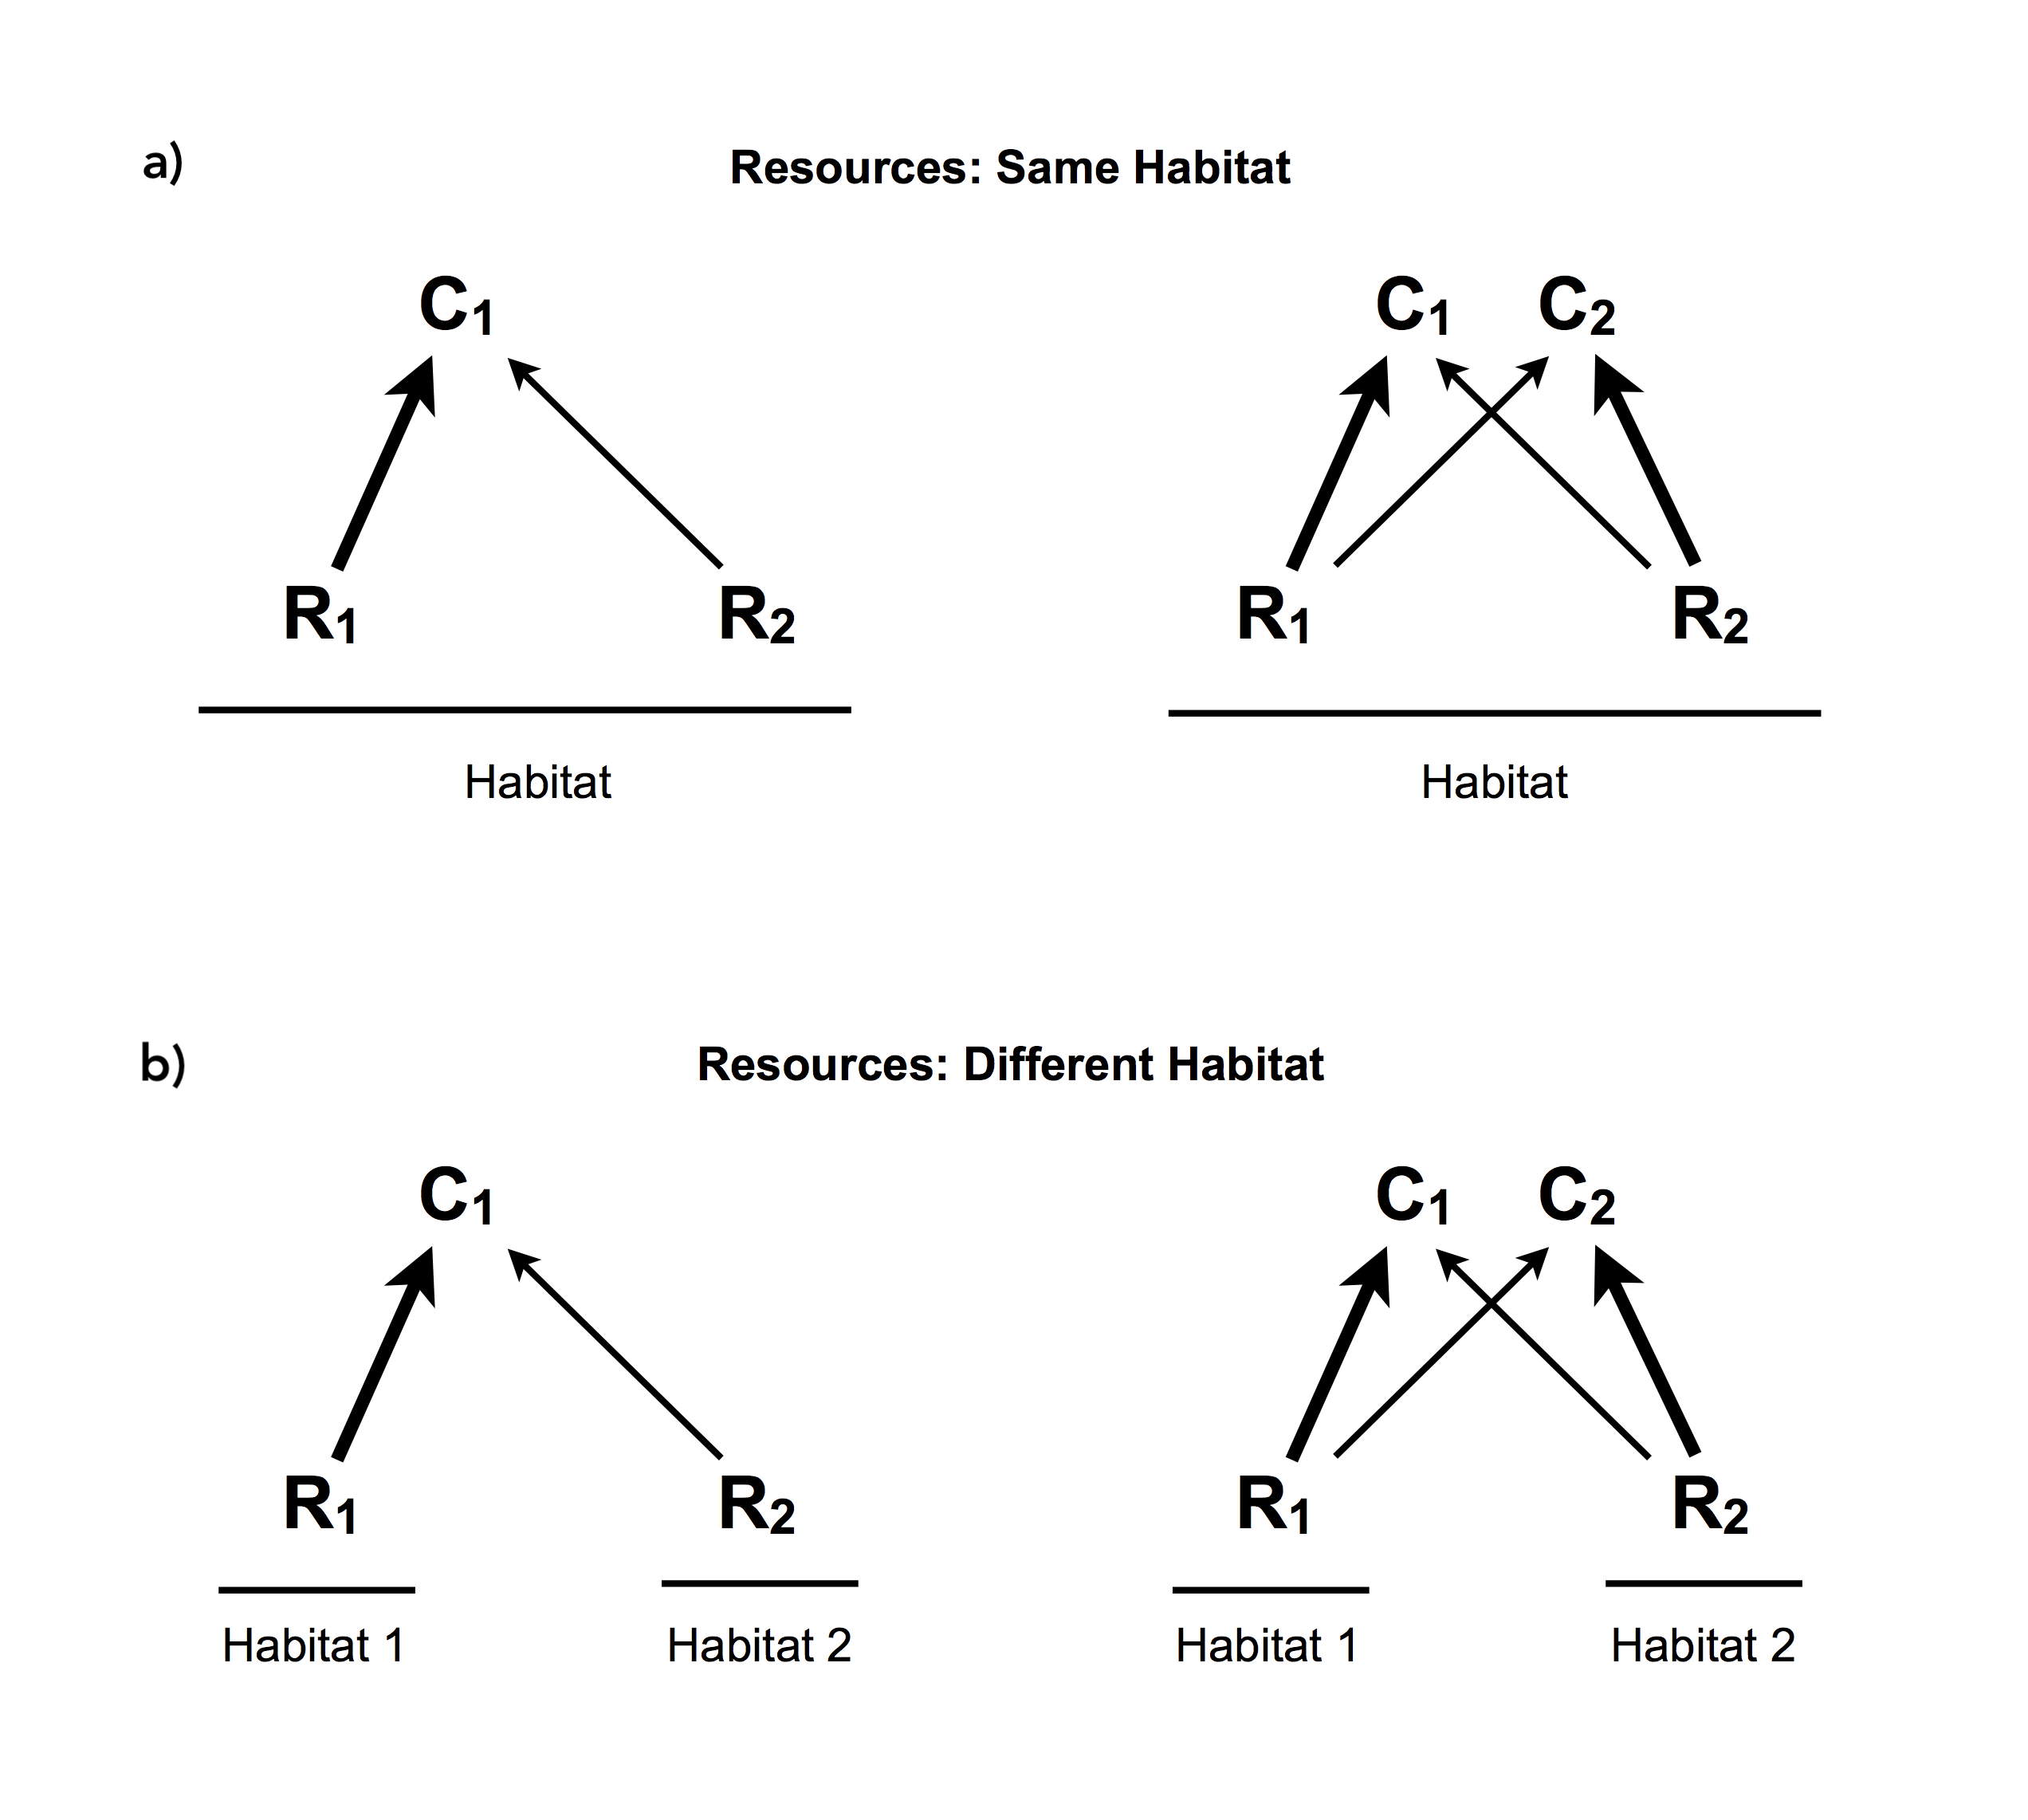
\includegraphics{Fig_1_ForagingScenarios}
\caption{\label{fig:foraging_scenarios}\textbf{Ecological foraging
scenarios.} I examined whether the effect of ecological character
displacement on food-web dynamics depended on whether consumers competed
for resources that occurred in the same (a) vs.~different habitats (b).
Note that inferences about character displacement can only be made by
comparing food webs with (right) and without (left) a competing
consumer, so I arbitrarily set \emph{C}\textsubscript{2} = 0 for these
comparisons. The width of each arrow corresponds to the initial attack
rate (\emph{a}\textsubscript{ij}) of consumer \emph{j} on resource
\emph{i}. Note that \emph{C}\textsubscript{1} was pre-adapted to
\emph{R}\textsubscript{1} (\emph{a}\textsubscript{11} \textgreater{}
\emph{a}\textsubscript{21}), while \emph{C}\textsubscript{2} was a
mirror image, being pre-adapted to \emph{R\textsubscript{2}}
(\emph{a}\textsubscript{22} = \emph{a}\textsubscript{11};
\emph{a}\textsubscript{12} = \emph{a}\textsubscript{21}). In each
scenario, I assumed consumer feeding rates increased linearly with
resource abundance. I also relax this assumption and consider a more
realistic functional response when resources occurred in different
habitats (b).}
\end{figure}

\subsection{Food-web dynamics}\label{food-web-dynamics}

Given that character displacement occurred across these foraging
scenarios, I focus here on its consequences for food-web dynamics. To do
this, I analyzed differences in resource abundances and food-web
stability at equilibrium. An equilibrium is reached when there is no
change in the population growth rates of consumers and resources (i.e.,
the rates of change in equation \ref{eq:1} are 0), and solving the
system at this point gives equilibrium abundances for each resource
(\(\hat R_i\)) and each consumer (\(\hat C_j\)). I also compared the
local stability of these food webs using standard methods
\citep{Otto2007}. This stability analysis derives the dominant
eigenvalue, \(\lambda_{\text{max}}\), of the matrix of partial
derivatives of each species' population growth rate (given by equation
\ref{eq:1}) with respect to each species' abundance evaluated at
equilibrium. If \(-\lambda_{max}>0\), then the food web will return to
equilibrium after a small perturbation (i.e., it is locally stable),
with more positive values indicating a faster return time. If
\(-\lambda_{max}<0\), then the food web is not locally stable.

When possible, I derived analytical expressions for the relationship
between consumer attack rates and food-web dynamics. To do this, I
simplified the model by assuming that resources are equivalent
(\(r=r_i\) and \(K=K_i\)) as well as consumers (\(e=e_{ij}\);
\(h=h_{ij}\); \(m=m_j\)), except that consumer attack rates and their
habitat preferences (if present) are mirror images of each other
(\(a_{11}=a_{22}\); \(a_{12}=a_{21}\); \(w_{11}=w_{22}\)). Note that I
arbitrarily set \(C_1\) as being pre-adapted to \(R_1\)
(\(a_{11} > a_{21}\); \(w_{11} > 0.5\)), and therefore \(C_2\) was
pre-adapted to \(R_2\). Controlling for other sources of variability
allowed me to isolate the general effects of character displacement. All
mathematical derivations were conducted in Mathematica
\citep{Mathematica} and are provided in Appendices S1-3.

To gain insight to the eco-evolutionary feedback generated by character
displacement, I conducted simulations using an Adaptive Dynamics
approach. Specifically, after letting consumer and resource abundances
reach a steady state, I created a mutant consumer by randomly choosing
one and modifying its attack rate on one resource by either subtracting
or adding a small constant (0.01 in the following simulations) with
equal probability. The mutant's attack rate on the other resource was
determined by a tradeoff, such that
\(\big(a_{\text{1},j}/{A}\big)^n+\big(a_{\text{2},j}/{A}\big)^n=1\),
where \(A\) is the total investment in attack rates and \(n\) describes
the shape of the tradeoff \citep{Sargent2006}. This function has the
useful property that it differentiates between cases where intermediate
combinations of \(a_{\text{1},j}\) and \(a_{\text{2},j}\) are higher
than the extremes (when \(n>1\), green line in Fig. \ref{fig:tradeoff})
or, conversely, where the two extremes are higher than intermediate
investments (when \(n<1\), orange line in Fig. \ref{fig:tradeoff}). When
\(n=1\), the tradeoff function is linear, and all combinations of
\(a_{\text{1},j}\) and \(a_{\text{2},j}\) have the same total attack
rate (blue line in Fig. \ref{fig:tradeoff}). Assuming the mutant
consumer was rare, I then determined whether the mutant had higher
relative fitness than the resident consumer, and thus could invade and
replace the resident consumer. If the mutant was able to invade, I
updated the attack rate of the resident consumer to the mutant attack
rate and allowed consumer and resource abundances to reach a steady
state. I then repeated the simulation up to 10,000 times, which was
sufficient for consumers to either reach an evolutionary stable strategy
\citep[ESS,][]{Smith1973} or an evolutionary limit (e.g.,
\(\frac{a_{ij}}{a_{\text{1},j}+a_{\text{2},j}}\) is constrained to a
maximum of 1 and minimum of 0). Unless otherwise noted, I conducted
simulations with the following parameter values: \emph{r} = 1; \emph{K}
= 4; \emph{e} = 0.8; \emph{m} = 1; \emph{A} = 2; \emph{h} = 0.4; and
\(w_{11} = w_{22} = 0.6\). I set an initial value of
\(a_{11} = a_{22} = 1.2\), while \(a_{12}\) and \(a_{21}\) depended on
the value of \emph{n}. I set initial consumer and resource abundances
to: \(R_1 = R_2 = 2\); \(C_1 = C_2 = 1\). All simulations were conducted
in R \citep{R} and the code to reproduce these simulations is publically
available on GitHub (\url{https://github.com/mabarbour/ECD_model}).

\begin{figure}
\centering
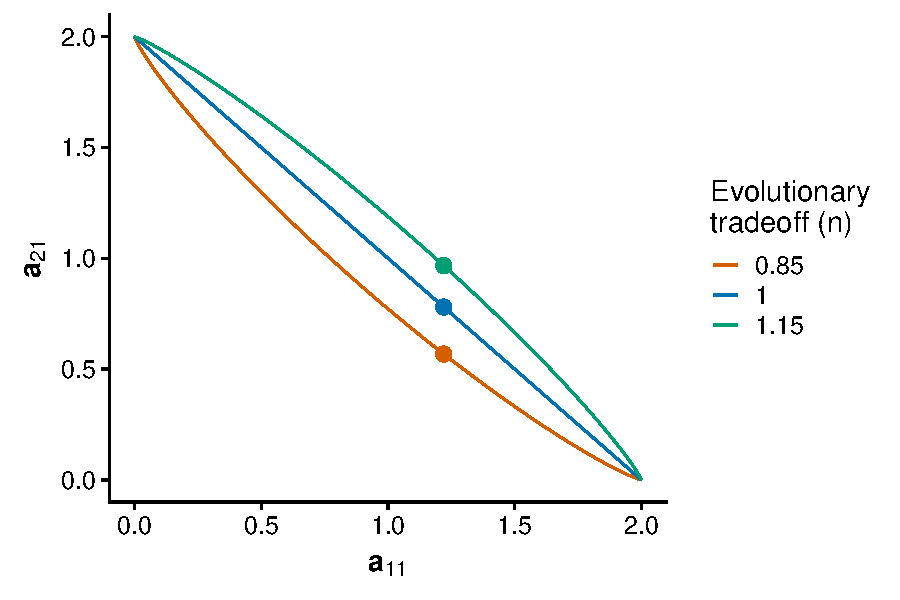
\includegraphics{Fig_2_Tradeoffs.pdf}
\caption{\label{fig:tradeoff}\textbf{Evolutionary tradeoffs in consumer
attack rates.} In each foraging scenario, I explored the effects of
three different tradeoffs: intermediate combinations of attack rates
(\emph{a}\textsubscript{1,\emph{j}}, \emph{a}\textsubscript{2,\emph{j}})
are higher than the extremes (green line, \emph{n} \textgreater{} 1);
extreme combinations of attack rates are higher than intermediate
investments (orange line, \emph{n} \textless{} 1); and all combinations
of attack rates have the same total attack rate (blue line, \emph{n} =
1). Points corresponding to attack rates at the beginning of the
simulation for \emph{C}\textsubscript{1}, which was pre-adapted to
\emph{R}\textsubscript{1} (\emph{a}\textsubscript{11} \textgreater{}
\emph{a}\textsubscript{12}). Note that \emph{C}\textsubscript{2} was a
mirror image of \emph{C}\textsubscript{1}, being pre-adapted to
\emph{R}\textsubscript{2} (\emph{a}\textsubscript{22} =
\emph{a}\textsubscript{11}; \emph{a}\textsubscript{12} =
\emph{a}\textsubscript{21}).}
\end{figure}

\section{Results}\label{results}

\subsection{Resources occur in the same
habitat}\label{resources-occur-in-the-same-habitat}

In this first scenario (equation \ref{eq:2}), the abundance of resources
at equilibrium are equivalent when both consumers and resources are
present (\(\hat R = \hat R_1 = \hat R_2\)), and are determined by the
following equation (derived in Appendix S2):

\begin{equation} \label{eq:5}
  \hat{R}=\frac{1}{a_{1,j}+a_{2,j}}\cdot\frac{m}{e}
\end{equation}

A key determinant of resource abundance in this scenario is the
consumer's total attack rate, \(a_{1,j}+a_{2,j}\). Therefore, the effect
of character displacement on food-web dynamics depends on how the shape
of the tradeoff function influences the evolution of consumer attack
rates.

I found that the shape of the tradeoff function qualitatively affects
the relationship between character displacement and resource abundances
in this scenario (Fig. \ref{fig:plot_fig3}a,b). For example, if
consumer's are constrained by a linear tradeoff (blue lines), then there
is no net change in total attack rate (Fig. \ref{fig:plot_fig3}a) and
character displacement has no effect on resource abundances (Fig.
\ref{fig:plot_fig3}b). If the tradeoff is concave down (green lines),
then resource abundances can actually increase under character
displacement (Fig. \ref{fig:plot_fig3}b). This is because the total
attack rate of consumers is maximized at intermediate values
(\(a_{1,j}=a_{2,j}\)) and decreases as consumers diverge (Fig.
\ref{fig:plot_fig3}a). When the tradeoff is concave up (orange lines),
character displacement suppresses resource abundances due to the
increase in total attack rates (Fig. \ref{fig:plot_fig3}a,b). Although
the equation I derived for resource abundances was for the scenario
where both consumers and both resources were present, it accurately
predicts the abundance of resources when a single consumer reaches its
evolutionary stable strategy (ESS; triangles on respective colored lines
in Fig. \ref{fig:plot_fig3}b). This is because a single consumer evolves
to be a generalist that has equal attack rates on each resource
(triangles at 0.5 along x-axis in Fig. \ref{fig:plot_fig3}a), resulting
in equivalent resource abundances.

The effect of character displacement on resources corresponds to its
impact on food-web stability. For example, when character displacement
decreases resource abundances (orange points in Fig.
\ref{fig:plot_fig3}b), there is also a decrease in food-web stability
(Fig. \ref{fig:plot_fig3}c). Character displacement may not affect or
even increase food-web stability (blue and green lines in Fig.
\ref{fig:plot_fig3}c); however, evolution does not favor strong
divergence in these scenarios (blue and green points in Fig.
\ref{fig:plot_fig3}a), which dampens these contingent effects. Note that
the dip in stability occurs when both consumers evolve to be
generalists, a situation that is not favored in any of the foraging
scenarios I examined (Fig. \ref{fig:plot_fig3}c).

\subsection{Resources occur in different
habitats}\label{resources-occur-in-different-habitats}

In the second foraging scenario (equation \ref{eq:3}), I again see that
resource abundances are equivalent when both consumers and resources are
present (\(\hat R = \hat R_1 = \hat R_2\)), but are now determined by
the following equation (derived in Appendix S3):

\begin{equation} \label{eq:6}
  \hat{R}=\frac{1}{w_{1,j}a_{1,j}+w_{2,j}a_{2,j}}\cdot\frac{m}{e}
\end{equation}

This equation implies that if consumers evolve to become specialists on
resources that occur in their preferred habitat (e.g., \(w_{1,j}>0.5\)
and \(a_{1,j}>a_{2,j}\)), then the effective attack rate of consumers
(\(w_{1,j}a_{1,j}+w_{2,j}a_{2,j}\)) will always increase, regardless of
the tradeoff (Fig. \ref{fig:plot_fig3}d). Thus, character displacement
always results in resource suppression (Fig. \ref{fig:plot_fig3}e). Note
that the shape of the tradeoff can modify the effect of character
displacement. This is not so much due to the tradeoff affecting the
magnitude of displacement (it does, but the effect is minor), but
because the form of the tradeoff affects resource abundances when a
single consumer has reached an ESS (triangles in Fig.
\ref{fig:plot_fig3}e). In contrast, resource abundances reach a similar
value when consumers evolve in the presence of a competitor (circles in
Fig. \ref{fig:plot_fig3}e), because character displacement tends to
reach a constraint of complete specialization. It is worth noting that
resource abundances are consistently higher at the single consumer ESS
compared to the predictions I derived for when both consumers are
present (deviation of triangles from respective colored lines in Fig.
\ref{fig:plot_fig3}e). This is because consumers actually evolve
slightly specialized attack rates on the resources that occur in their
non-preferred habitat (deviation of triangles from 0.5 along x-axis in
Fig. \ref{fig:plot_fig3}d).

As seen previously, the effect of character displacement on resource
abundances qualitatively corresponds to its effect on food-web stability
(Fig. \ref{fig:plot_fig3}f). Specifically, character displacement
decreases food-web stability, regardless of the tradeoff in attack
rates. This is not simply a consequence of having an additional consumer
in the system, but emerges from the eco-evolutionary feedback between
character displacement and resource suppression (Fig.
\ref{fig:plot_fig3}c). For example, when the tradeoff is concave up
(orange), the initial two-consumer food web (small circle) is more
stable than when there is only one consumer (small triangle); however,
this pattern switches by the end of the eco-evolutionary simulation
(large points).

\begin{figure}
\centering
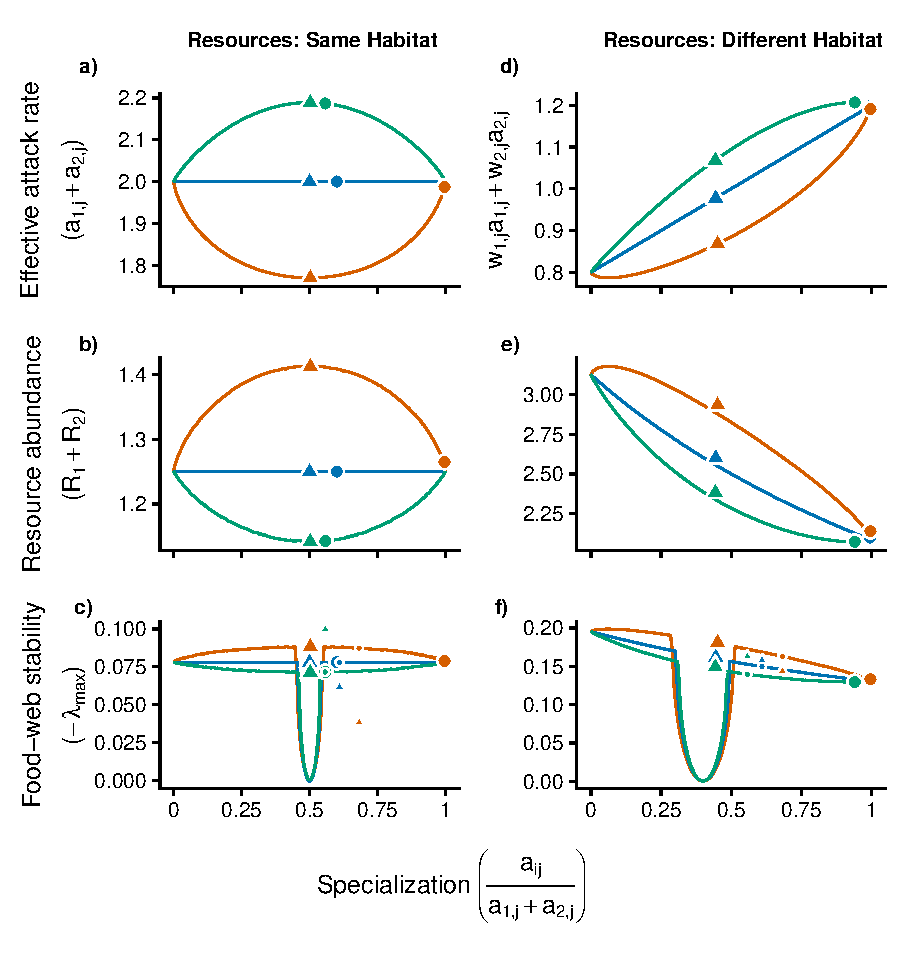
\includegraphics{Fig_3_MacArthur_LawlorSmith.pdf}
\caption{\label{fig:plot_fig3}\textbf{Effect of character displacement
on food-web dynamics under different evolutionary tradeoffs and foraging
scenarios.} Lines show predicted values when both consumers and
resources are present. Different line colors correspond to different
tradeoffs in attack rates (green, \emph{n} = 1.15; blue, \emph{n} = 1;
orange, \emph{n} = 0.85). Large circles (two consumers) and triangles
(one consumer) correspond to the end points of the eco-evolutionary
simulation for \emph{C}\textsubscript{1} (the choice to display
\emph{C}\textsubscript{1} was arbitrary), whereas as small shapes
correspond to the starting points (only in stability panels). In both
foraging scenarios, feeding rates increase linearly with resource
abundance, but the equation for the effective attack rate is different.}
\end{figure}

\subsection{Adding a more realistic functional
response}\label{adding-a-more-realistic-functional-response}

In the third foraging scenario (equation \ref{eq:4}), I observed the
same general effect of character displacement as the previous scenario
(resources in different habitats, but linear functional response). This
is because resource abundances at equilibrium are governed by a similar
dynamic (derived in Appendix S1):

\begin{equation} \label{eq:7}
  \hat{R}=\frac{1}{w_{1,j}a_{1,j}+w_{2,j}a_{2,j}}\cdot\frac{m}{e-hm}
\end{equation}

And since evolution favors character displacement toward their preferred
resources (see Appendix S1), the effective attack rate of consumers
(\(w_{1,j}a_{1,j}+w_{2,j}a_{2,j}\)) will always increase, resulting in
lower resource abundances and decreased food-web stability (Appendix S4,
Fig. S1).

In the first two foraging scenarios, character displacement influences
food-web stability, but all of the food webs ultimately return to a
stable equilibrium (because \(-\lambda_{max}>0\), see Appendix S2-3). In
this more realistic model, however, whether the food web is locally
stable depends on consumer and resource parameters. Specifically, I
found that the two-consumer food web will transition from having a
locally stable equilibrium to a limit cycle under the following
conditions (derived using Routh-Hurwitz criteria in Appendix S1):

\begin{equation} \label{eq:8}
  w_{1,j}a_{1,j}+w_{2,j}a_{2,j} > \frac{e+hm}{hK(e-hm)}
\end{equation}

This inequality indicates that character displacement always pushes the
food web toward an unstable structure in this more realistic foraging
scenario (Fig. \ref{fig:bifur_plot}). Note that I stopped the simulation
in the two-consumer food web once it became locally unstable. I do not
simulate beyond this point as this would require making assumptions
about the dynamics of mutant consumers in variable environments, which
is beyond the scope of this work.

\begin{figure}
\centering
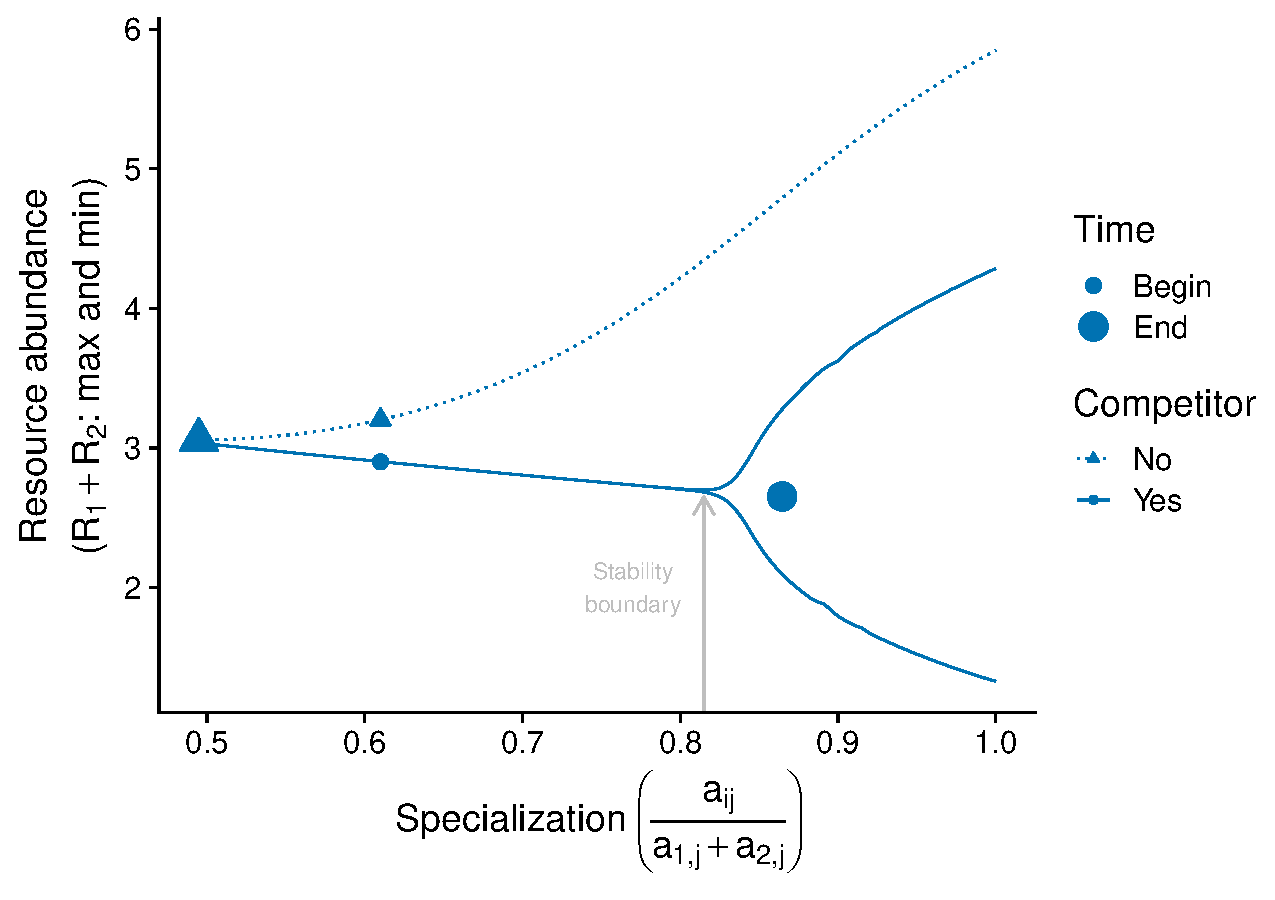
\includegraphics{Fig_4_Bifurcation.pdf}
\caption{\label{fig:bifur_plot}\textbf{Character displacement creates an
unstable food web}. Lines illustrate the effect of character
displacement across the range of specialization for
\emph{C}\textsubscript{1} (the choice to display
\emph{C}\textsubscript{1} was arbitrary), while the points are the
results of an eco-evolutionary simulation. Note that I increased the
total investment in attack rates (\emph{A} = 3.3) to create a scenario
that could result in an unstable food web. Although I specified a linear
tradeoff in attack rates for this simulation, different tradeoff shapes
do not qualitatively alter these results (see Appendix S4, Fig. S1).}
\end{figure}

\subsection{Robustness to consumer
asymmetry}\label{robustness-to-consumer-asymmetry}

The previous analytical results and simulations make a strong assumption
that competing consumers start off as perfect mirror images of each
other (i.e., there is symmetry). Yet, theory indicates a predictable
asymmetry between initial consumer attack rates. This predictable
asymmetry emerges from a process of community assembly where a single
consumer invades a system, evolves to be a generalist that can equally
attack both resources, followed by the invasion of a second, more
specialized, consumer. This theoretical scenario has been hypothesized
as the sequence of events leading to character displacement in
threespine stickleback in small coastal lakes of British Columbia
\citep{Schluter1992, Schluter2000}.

To test whether my results were robust to this asymmetry, I used the
evolved attack rates at the end of the simulations with one consumer as
the starting values for one of the two consumers. I did this for all
foraging scenarios and tradeoffs previously examined. I found that my
previous inferences are robust to including consumer asymmetry across
different foraging scenarios and tradeoffs (Appendix S4, Fig. S2-3).

\section{Discussion}\label{discussion}

\subsection{Resource abundances}\label{resource-abundances}

One of the criteria used to demonstrate ecological character
displacement is that ``sites of sympatry {[}two consumers{]} and
allopatry {[}one consumer{]} should not differ greatly in food
\(\textbf{[}\)resource abundances\(\textbf{]}\)'' \citep{Schluter1992}.
In contrast, my results indicate that character displacement causes
predictable differences in resource abundances. In fact, the ecological
and evolutionary scenarios that favored the largest character
displacement always decreased the relative abundance of resources. For
example, if mobile consumers compete for resources that occur in
different habitats, then character displacement always resulted in lower
resource abundances. Threespine stickleback, one of the classic examples
of character displacement, exemplify this foraging scenario
\citep{Schluter1992, Schluter2000}. Stickleback must move between the
pelagic and littoral zones of a lake when foraging for zooplankton and
benthic invertebrates, respectively. The theory developed here predicts
that resource abundances will be lower in lakes where competing
stickleback have undergone character displacement compared to lakes with
only a single species of stickleback. Interestingly, a disproportionate
number of the documented cases of character displacement involve
carnivores \citep{Schluter2000} that are larger, and likely more mobile,
than their resources \citep{McCann2005}, suggesting that many cases of
ecological character displacement may result in lower resource
availability.

Similarly, the evolutionary tradeoff that favored character displacement
decreased resource availability across all foraging scenarios. Although
data on the shape of the tradeoff in consumer foraging traits is scarce,
two classic examples of character displacement, Darwin's finches and
threespine stickleback, both appear to exhibit a tradeoff where extreme
trait values increase the net foraging rate of consumers
\citep{Schluter1985, Arnegard2014}. While it is theoretically possible
that character displacement does not alter (or even increase) resource
abundances, this was limited to the simplest, and arguably least
realistic, foraging scenario and under tradeoffs that did not favor
large displacements, and thus less likely to detect in nature. Taken
together, my results call for empirical work to test these clear
theoretical predictions and suggest a revision is needed for one of the
criteria used to demonstrate character displacement.

\subsection{Food-web stability}\label{food-web-stability}

My most striking result was that ecological character displacement made
food webs less resilient to perturbations. In fact, under the most
realistic foraging scenario, character displacement can even result in
an unstable food web. The mechanism underlying this destabilization is
quite general. Character displacement generally increases the strength
of consumer-resource interactions, but does not alter the strength of
intraspecific interactions. This relative increase in interspecific
interactions, combined with the natural oscillatory tendency of
consumer-resource dynamics \citep{Lotka1925, Volterra1926}, creates a
food-web structure that is less resilient to perturbations
\citep{Chesson2008, Rip2011, McCann2011}.

Interestingly, the ecological conditions that favor character
displacement are those that are already the least resilient to
perturbations. For example, \citet{McPeek2019} showed that character
displacement is favored in food webs that are either highly productive,
easy to find and capture resources, or under weak abiotic stress. This
corresponds to higher values of \(K\) (productivity) or \(A\)
(investment in attack rates), or lower values of \(m\) (abiotic stress).
Each of these corresponding changes decrease food-web resilience, as
they increase the strength of consumer-resource interactions relative to
intraspecific interactions. For example, increasing productivity reduces
intraspecific competition in resource populations while increasing the
flux of energy to consumers, resulting in the paradox of enrichment
\citep{Rosenzweig1971}. Similarly, higher feeding rates or lower
consumer mortality both increase the relative strength of
consumer-resource interactions, which predictably destabilizes food webs
\citep{Rip2011, McCann2011}. This suggests that the most dramatic
examples of character displacement will not only occur in, but also
cause, the least stable food-web structures.

A handful of empirical patterns support the hypothesis that character
displacement decreases food-web resilience. For example, a single
species of threespine stickleback lives in hundreds of small coastal
lakes in British Columbia, but the species pair, where character
displacement has resulted in specialized limnetic and benthic species,
are only known from six lakes in four independent watersheds
\citep{Schluter1992, Schluter2000}. Perhaps many lakes had a species
pair in the past, but have lost a species due to a less resilient
food-web structure \citep{Borrelli2015a, Borrelli2015b}. The species
pair are known to be vulnerable to perturbations, as they have gone
extinct in two of the six lakes after the introduction of nonnative
species \citep{Hatfield2001, Taylor2006, Rudman2016}. The vulnerability
of the stickleback system also corresponds with the fact that aquatic
food webs have several properties that make them less resilient to
perturbations, such as higher productivity and more efficient energy
transfer to consumers \citep{Rip2011}. Detecting the ghost of
competition past \citep{Connell1980} may be quite difficult, but it
could be possible with recent advances in genomics. For example,
\citet{Feulner2018} detected genomic signatures of hybridization in
sympatric whitefish species following periods of eutrophication. Perhaps
solitary stickleback in some lakes retain genomic signatures of having
been a habitat specialist in the past.

My results contrast, but do not necessarily contradict, the notion from
coexistence theory that character displacement contributes to species
coexistence \citep{Lawlor1976}. Rather than studying resilience,
coexistence theory usually studies the mutual ability of consumers with
different phenotypes to invade when rare \citep[i.e., mutual
invasibility;][]{Chesson2000}. In the context of character displacement,
a shortcoming of this mutual invasibility measure is that it does not
allow a comparison between food webs with and without a competing
consumer. Such comparisons are necessary for inferring the effects of
character displacement, a point that has been made clear in the criteria
to demonstrate character displacement
\citep{Schluter1992, Schluter2000}. Although the addition of a consumer
to a food web can decrease its resilience in the absence of evolution
\citep{May1973}, my results are primarily driven by an eco-evolutionary
feedback between consumer evolution and resource abundances.

\subsection{Caveats}\label{caveats}

Although I model the indirect effects of coevolution between consumers,
I do not account for potential coevolution between consumers and
resources. In the context of my model, I would expect prey to evolve
traits that reduce consumer attack rates. Thus, prey evolution would act
to counter the effects of character displacement on resource abundance
and food-web stability. Note that this does not negate my general
conclusion that ecological character displacement decreases resource
abundances and stability; however, this process may itself create
another eco-evolutionary feedback between consumers and resources. This
may actually help maintain dramatic examples of character displacement
and prevent them from destabilizing systems, because it allows consumer
traits to become decoupled from their attack rate. Examining this
decoupling would be ideal in a quantitative genetic model that
explicitly tracks trait dynamics, but it would not fundamentally change
the conclusions presented here.

Another potential caveat is that I explored my model in a setting that
makes many assumptions about resource and consumer symmetry (but see
consumer asymmetry section). Prior work has shown that allowing for
resource asymmetry, for example, may decrease the magnitude of character
displacement \citep{Abrams1986}. While this may dampen the amount of
divergence, it should not qualitatively change the relationship I
observed.

I studied this eco-evolutionary feedback between consumers and resources
using an Adaptive Dynamics approach. A strength of this approach is that
it enabled me to gain analytical insight to the effects of character
displacement in a more realistic foraging scenario. This is much less
tractable in quantitative genetic \citep{Taper1985, McPeek2017} or
explicit genetic \citep{Doebeli1996} models of character displacement,
which is why the foraging scenarios previously examined have been
limited \citep[but see][]{McPeek2017}. A weakness, however, is that I
assume a separation of time scales between ecological and evolutionary
dynamics, an assumption that is becoming less tenable
\citep{Hairston2005, Hendry2016}. I also do not explicitly model an
underlying phenotypic trait for consumer attack rates nor do I allow for
intraspecific variation. That being said, my theoretical predictions are
likely robust to these assumptions. This is because models that
explicitly include resource dynamics inevitably show that resource
competition results in character displacement, regardless of whether a
quantitative genetic or Adaptive Dynamics approach is used
\citep{Lawlor1976, Taper1985}. A quantitative genetic model may
certainly show differences in the pace of character displacement, but
this should not qualitatively change its effect on food-web dynamics. It
is important to note that my conclusions only apply to food webs with
biotic resources that are nutritionally substitutable. It would be
interesting to extend these current analyses to non-substitutable
resources where convergent character displacement is expected
\citep{Abrams1987, Fox2008}.

\subsection{Conclusions}\label{conclusions}

Here, I show that an adaptive process that generates phenotypic
diversity generally makes that diversity more susceptible to future
extinctions. This destabilizing effect emerges from an eco-evolutionary
feedback involving direct and indirect interactions between species in a
food-web context. This result contrasts with the current notion that
patterns of phenotypic diversity are solely the result of evolutionary
constraints imposed by mutation, natural selection, gene flow, and
genetic drift. In particular, my result supports the recent suggestion
that food-web stability can impose an ecological constraint on
phenotypic diversity that is agnostic to these evolutionary processes
\citep{Borrelli2015b}. I expect that identifying when and where this
ecological constraint arises will yield novel insight to the patterns of
biodiversity we see in nature.

\section{Acknowledgements}\label{acknowledgements}

This work was inspired by discussions with Seth Rudman, Dolph Schluter,
Ben Gilbert, and Kevin McCann. Sally Otto provided much help in early
analyses of the mathematical model. I would not have been able to take
the theory as far as I did without her guidance and encouragement. Matt
Osmond, Jean Gibert, and Seth Rudman provided critical feedback on an
earlier draft. For funding support, I thank the University of British
Columbia (Four-Year Fellowship to M.A.~Barbour), NSERC (Discovery grant
to Greg Crutsinger), and the Swiss National Science Foundation (grant
31003A\_160671 to Jordi Bascompte).

\bibliography{ReferencesAbbrev}


\end{document}
